\documentclass[12]{beamer}

\usepackage[russian]{babel}
\usepackage{tikz}


\usetheme[progressbar=frametitle]{metropolis}
\setbeamertemplate{frame numbering}[fraction]
\usefonttheme{metropolis}
\setbeamercolor{background canvas}{bg=white}


\title{Семинар 7}
\subtitle{Магнитный момент. Спин. Сложные атомы}
\author{}
\date{\today}
\institute {\large 
\textbf{Ключевые слова}: магнитный и механический момент, спин, опыт Штерна-Грелаха, принцип Паули,  g-фактор, тонкое и сверхтонкое расщепление\\[6pt] 

\\[6pt] 
\textbf{Задачи}: 6.9, 6.15, 6.76\\[6pt] 

}


\begin{document}
\metroset{block=fill}
\maketitle


\begin{frame}[t]{Связь магнитного и механического моментов}
\begin{columns}[onlytextwidth]
\column{0.55\textwidth}
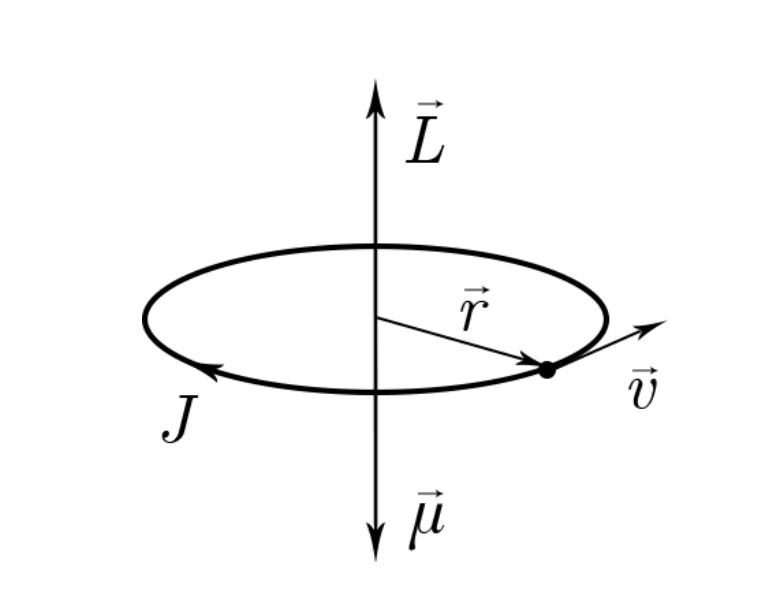
\includegraphics[width=\textwidth]{Seminar_07/pics/pic_01.PNG}
\column{0.45\textwidth}
Механический и магнитный моменты для электрона
\begin{gather*}
    \textbf{L} = [\textbf{r} \times m\textbf{v}] = rmv \textbf{n}\\
    \mu = \dfrac{J\textbf{S}}{c} = \dfrac{1}{c} \dfrac{ev}{2\pi r}\pi r^2 \textbf{n} = \\= - \dfrac{e}{2c} rv\textbf{n} \dfrac{m}{m} = -\dfrac{e}{2mc}\textbf{L}
\end{gather*}
\end{columns}
\begin{block}{Общий вид этой связи}
\begin{equation*}
\mu = -g\cdot \dfrac{e\hbar}{2mc} m_z = -g \mu_{\text{Б}} m_z   
\end{equation*}
$g$ -- фактором Ланде, $\mu_{\text{Б}} = 927 \cdot 10^{-26} \frac{\text{Дж}}{\text{Тл}} = 0.927 \cdot 10^{-20} \frac{\text{эрг}}{\text{Гс}}$ -- магнетон Бора
\end{block}
\end{frame}

\begin{frame}[t]{Экспериментальное подтверждение связи  моментов}
\begin{block}{Опыт Эйнштейна - де Гааза}
\centering
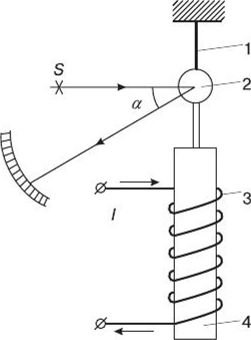
\includegraphics[width=0.4\textwidth]{Seminar_07/pics/pic_de_gaaz.png}
\\
Оценка эффекта:
$I\omega = N\cdot 2L_{e}$\\
Для цилиндра массой 100 грамм и радиусом 1 см, характерная угловая скорость получается около $10^{-3}$ Гц
\end{block}
\end{frame}

\begin{frame}[t]{Экспериментальное подтверждение связи  моментов}
\begin{block}{Опыт Штерна Герлаха}
\centering
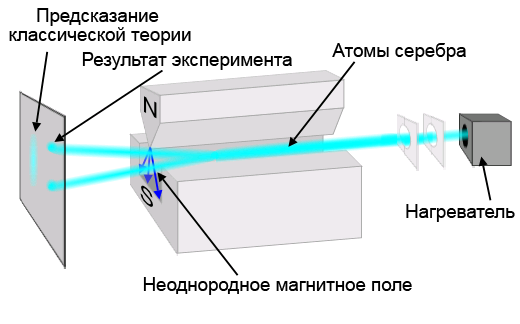
\includegraphics[width=0.6\textwidth]{Seminar_07/pics/pic_02.png}
\\
Мультиплетность $2S+1=2 \Rightarrow S = \pm \dfrac{1}{2}$ -- это спин 

Как следствие -- 4 квантовых числа для атома 
\end{block}
\end{frame}


\begin{frame}[t]{Сложение моментов}
\only<1>{
\begin{block}{2 момента импульса}
у нас есть 2 момента $L_1, L_2$ этому соответствует проекций на выбранную ось для этих операторов будут $l_1, l_2; l_1>l_2$. Максимальная проекция момента будет их суммой $l_1 + l_2$, когда их направления совпадают, а минимально возможная проекция равна их разности $l_1 - l_2$, когда они направлены в разные стороны. Всего состояний:
\begin{equation*}
    N_{tot} = \sum\limits_{l=l_1-l_2}^{l_1+l_2}2l+1 = (2l_1+1)(2l_2+1)
\end{equation*}
\end{block}
}
\only<2>{
\begin{block}{Полный момент}
Орбитальный момент $L$ и спиновый момент $S$. Для них магнитные моменты:
\begin{gather*}
    \mu_l = -g_l\mu_{\text{Б}}l\\
    \mu_s = -g_s\mu_{\text{Б}}s\\
    J = L+S\\
    \mu_j = -g_j\mu_{\text{Б}}j\\
\end{gather*}
Ответ для суммарного g-фактора:
\begin{equation*}
    g_j = 1+\dfrac{J(J+1) + S(S+1) - L(L+1)}{2J(J+1)} 
\end{equation*}
\end{block}
}
\end{frame}

\begin{frame}[t]{Сложный атом}
\only<1>{\begin{block}{Терм}
\begin{equation*}
    n^{2S+1}L_J
\end{equation*}
Для основного состояния натрия $1s^22s^22p^63s^1 \Rightarrow 3^1S_{\frac{1}{2}}$
\end{block}
}
\only<2>{
\begin{block}{Правила заполнения орбиталей}
\textit{Принцип запрета Паули.} Электроны, как частицы с полуцелым спином, фермионы, не могут существовать в одном энергетическом состоянии со всеми одинаковыми квантовыми числами. \\
\textit{Правила Хунда.} Это эмпирический набор правил заполнения энергетических оболочек атомов:
\begin{enumerate}
    \item Мультиплетность ($2S+1$) максимальна
    \item При совпадении мультиплетностей суммарный орбитальный момент $L$ максимален
\end{enumerate}

\end{block}
}
\end{frame}

\begin{frame}[t]{Тонкое и сверхтонкое расщепление}
\begin{block}{Тонкое расщепление}
Эффект <<барона Мюнхгаузена>>
\begin{gather*}
    \Delta U_{LS} \sim (\mu_S B_L) \sim  ( \hat{L}\hat{S} )\\
    \hat{J}=\hat{S}+\hat{L}\Rightarrow   \hat{J^2}=\hat{S^2}+\hat{L^2} + 2 (\hat{L}\hat{S})\\
    (\hat{L}\hat{S}) = \dfrac{1}{2} \left(\hat{J^2} -\hat{S^2} -\hat{L^2} \right) = \dfrac{1}{2} \left(J(J+1) -S(S+1) -L(L+1) \right)\\
\end{gather*}
\end{block}
\begin{block}{Сверхтонкое расщепление}
Связь спина ядра и спина электрона
\end{block}

\end{frame}




\begin{frame}{Задача 6.9}\scriptsize
\only<1>{\begin{block}{Условие}
С какой угловой скоростью $\omega$ и в каком направлении должен начать вращаться цилиндр, подвешенный магнитном поле $B$, направленном параллельно его оси вертикально вверх, если изменить направление поля на обратное? Считать, что цилиндр намагничивается до насыщения. Момент импульса электрона в атоме равен $k$, число атомов в
цилиндре $N$, момент инерции цилиндра $I$.
\end{block}}
\only<2>{\begin{block}{Решение}
Тут как и в теоретической части нужно приравнять момент импульса цилиндра как целого и момент импульса каждого отдельного атома:
\begin{equation*}
    I\omega = 2kN \Rightarrow \omega = \dfrac{2kN}{I}
\end{equation*}
\end{block}}
\end{frame}

\begin{frame}{Задача 6.15}\scriptsize
\only<1>{\begin{block}{Условие}
Параллельный пучок нейтронов с энергией $T = 0.025$ эВ проходит через коллимирующую щель шириной $ d= 0.1$ мм и затем через зазор в магните Штерна–Герлаха длиной $L = 1$ м. Оценить значение градиента поля $\frac{dB}{dz}$, при котором угол магнитного отклонения компонент пучка равен углу дифракционного уширения. Магнитный момент нейтрона $\mu_n = 9.66 \cdot 10^{−24}$ эрг/Гс.

\begin{figure}[h]
    \centering
    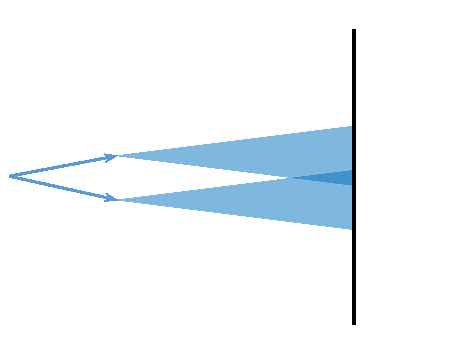
\includegraphics[width=0.5\textwidth,height=\textheight,keepaspectratio]{Seminar_07/pics/pic_03.pdf}
    \label{fig:sem_04}
\end{figure}
\end{block}}
\only<2>{\begin{block}{Решение}
Оценим дифракционное уширение:
\begin{equation*}
    \alpha_{\text{диф}}= \dfrac{\lambda}{d} = \dfrac{h}{d\sqrt{2mT}}
\end{equation*}
Рассчитаем отклонение под действием силы со стороны магнитного поля. Для этого разделим скорость на 2 компоненты продольную $v_{\parallel}$ и поперечную $v_{\perp}$ и свяжем их между собой. По сути это кинематическая задачка:
\begin{gather*}
    f_{\perp} =m a_{\perp} = \mu_n \dfrac{dB}{dz}; \Rightarrow a_{\perp} = \dfrac{\mu_n}{m} \dfrac{dB}{dz}\\
    v_{\perp} = a_{\perp} \tau, L=v_{\parallel}\tau; \Rightarrow v_{\perp} = \dfrac{\mu_n}{m} \dfrac{dB}{dz} \dfrac{L}{v_{\parallel}}\\
    \alpha_{\text{маг}}= \dfrac{v_{\perp}}{v_{\parallel}} = \dfrac{\mu_n \dfrac{dB}{dz} L}{mv^2_{\parallel}} \approx \dfrac{\mu_n \dfrac{dB}{dz} L}{2T}
\end{gather*}
По условию приравниваем углы отклонения между собой и получаем:
\begin{equation*}
    \dfrac{dB}{dz} = \dfrac{2Th}{L\mu_nd\sqrt{2mT}} \approx 150 \dfrac{\text{Гс}}{\text{см}}
\end{equation*}
\end{block}}
\end{frame}

\begin{frame}{Задача 6.76}\scriptsize
\only<1>{\begin{block}{Условие}
В спектрах газовых туманностей наблюдаются линии, которые долгое время не могли приписать ни одному из известных элементов. В последствии выяснилось, что это линии ионов кислорода и азота. Наиболее интенсивные линии соответствую переходам $^1D_2 \rightarrow ^3P_2$, $\lambda_1 = 5007$ \AA\text{ } и $^1D_2 \rightarrow ^3P_1$, $\lambda_2 = 4959$ \AA\text{ }для иона кислорода $O^{++}$. Найти длину перехода $^3P_1 \rightarrow ^3P_0$ с использованием схемы Рассела-Саундерса (LS-схема).\\
\begin{figure}[h]
    \centering
    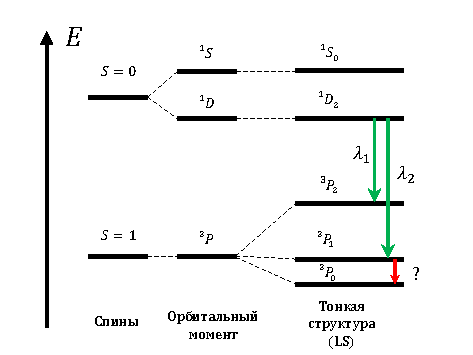
\includegraphics[width=0.6\textwidth,height=\textheight,keepaspectratio]{Seminar_07/pics/pic_04.pdf}
    \label{fig:sem_04}
\end{figure}
\end{block}}
\only<2>{\begin{block}{Решение}
\begin{equation*}
    E_{LS} = A(\hat{L}\hat{S} ) = \dfrac{A}{2}\left(J(J+1) - S(S+1) -L(L+1) \right)
\end{equation*}
Давайте с ее помощью запишем разность энергий этих уровней:
\begin{gather*}
    E(^3P_2) - E(^3P_1) = [E(^3P)+E_{LS}(J=2)] - [E(^3P)+E_{LS}(J=1)] =\\= \dfrac{A}{2}(2\cdot 3 - 1\cdot2)= 2A\\
    E(^3P_1) - E(^3P_0) = [E(^3P)+E_{LS}(J=1)] - [E(^3P)+E_{LS}(J=0)] = A\\
\end{gather*}
Теперь реализуем данные о переходах из условия:
\begin{gather*}
\begin{cases}
    E(^1D_2) - E(^3P_2) = \dfrac{hc}{\lambda_1}\\
    E(^1D_2) - E(^3P_1) = \dfrac{hc}{\lambda_2}
\end{cases}
\Rightarrow E(^3P_2) - E(^3P_1)= hc \dfrac{\lambda_1-\lambda_2}{\lambda_1\lambda_2} =2A
\end{gather*}
\end{block}}

\only<3>{
\begin{block}{Решение}
Далее аналогично 
\begin{gather*}
E(^3P_1) - E(^3P_0) = \dfrac{hc}{\lambda} = \dfrac{1}{2}(E(^3P_2) - E(^3P_1))= \dfrac{hc}{2} \dfrac{\lambda_1-\lambda_2}{\lambda_1\lambda_2}\\
\lambda = \dfrac{2\lambda_1\lambda_2}{\lambda_1-\lambda_2} \approx 0.01 \text{ см}
\end{gather*}
\end{block}
}
\end{frame}



\begin{frame}[t]{Комментарии к задачам из задания}\scriptsize
\begin{itemize}
\item Нулевки   Первая -- зная n надо найти l, m (привет табличке из прошлого семинара), вторая -- по известной конфигурацию найти l и s, 
\item Задача 6.10  Продолжение 6.9
\item Задача 6.15  Решена
\item Задача 6.20  Построить аналогичные 6.76 уровни энергии и учесть расщепление состояния $^2P$. Далее найти их разницу энергий, а эффективное поле из энергии выражается. Вспомните формулу из 3 семестра сами 
\item Задача 6.48  Можно рассмотреть взаимодействие спинов как взаимодействие магнитных диполей, поле от которых известно.
\item Задача 6.77  Повторят 6.76
\item Задача 6.78  Тут нужно заметить, что это обменное взаимодействие идет с разными знаками в зависимости от того орто это или пара гелий.
\item Задача Т2  Это задачка про перебор вариантов из решения 6.76
\end{itemize}
\end{frame}

\end{document}